\section{Simulation}
\begin{figure}[h]
    \centering
    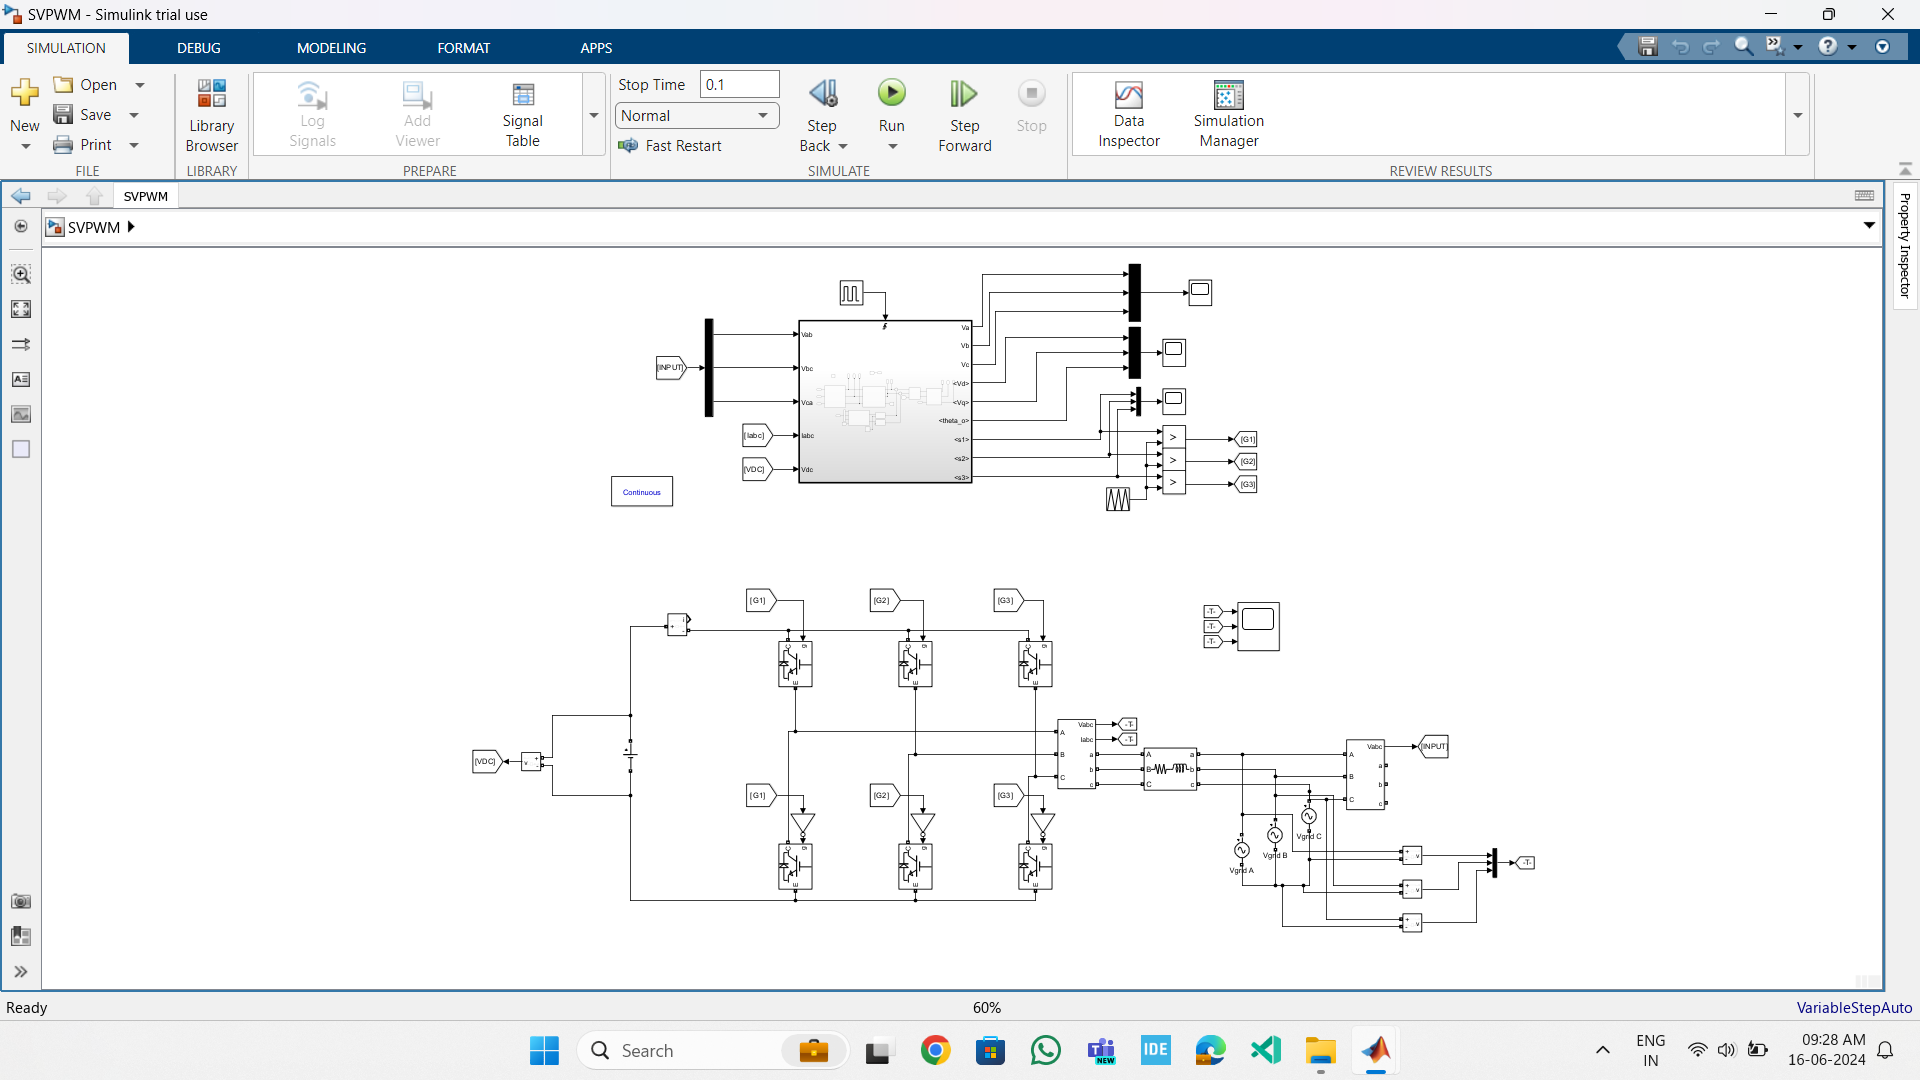
\includegraphics[width=\textwidth]{Whole Simulation.png}
    \caption{Simulation}
    \label{fig:Simulation}
\end{figure}
Before initiating the implementation phase, it was imperative to conduct a
comprehensive simulation of the front end using Simulink/MATLAB. The simulation
setup involved importing a three-phase source from MATLAB and configuring the
necessary parameters for voltage and current measurements.

\subsection{MATLAB Function Blocks in Simulation}
To emulate the behavior of a microcontroller in the simulation environment,
MATLAB function blocks were extensively utilized. These function blocks
provided a familiar coding environment, resembling the programming paradigms
employed in microcontroller firmware development. By encapsulating custom
algorithms and control logic within MATLAB function blocks, it was possible to
simulate complex control strategies and signal processing techniques with ease.
This approach not only facilitated rapid prototyping and testing but also
provided invaluable insights into the real-time behavior of the system. The use
of MATLAB function blocks bridged the gap between simulation and
implementation, enabling seamless transition from design validation to hardware
deployment.
\subsection{Control System}
\begin{figure}[h]
    \centering
    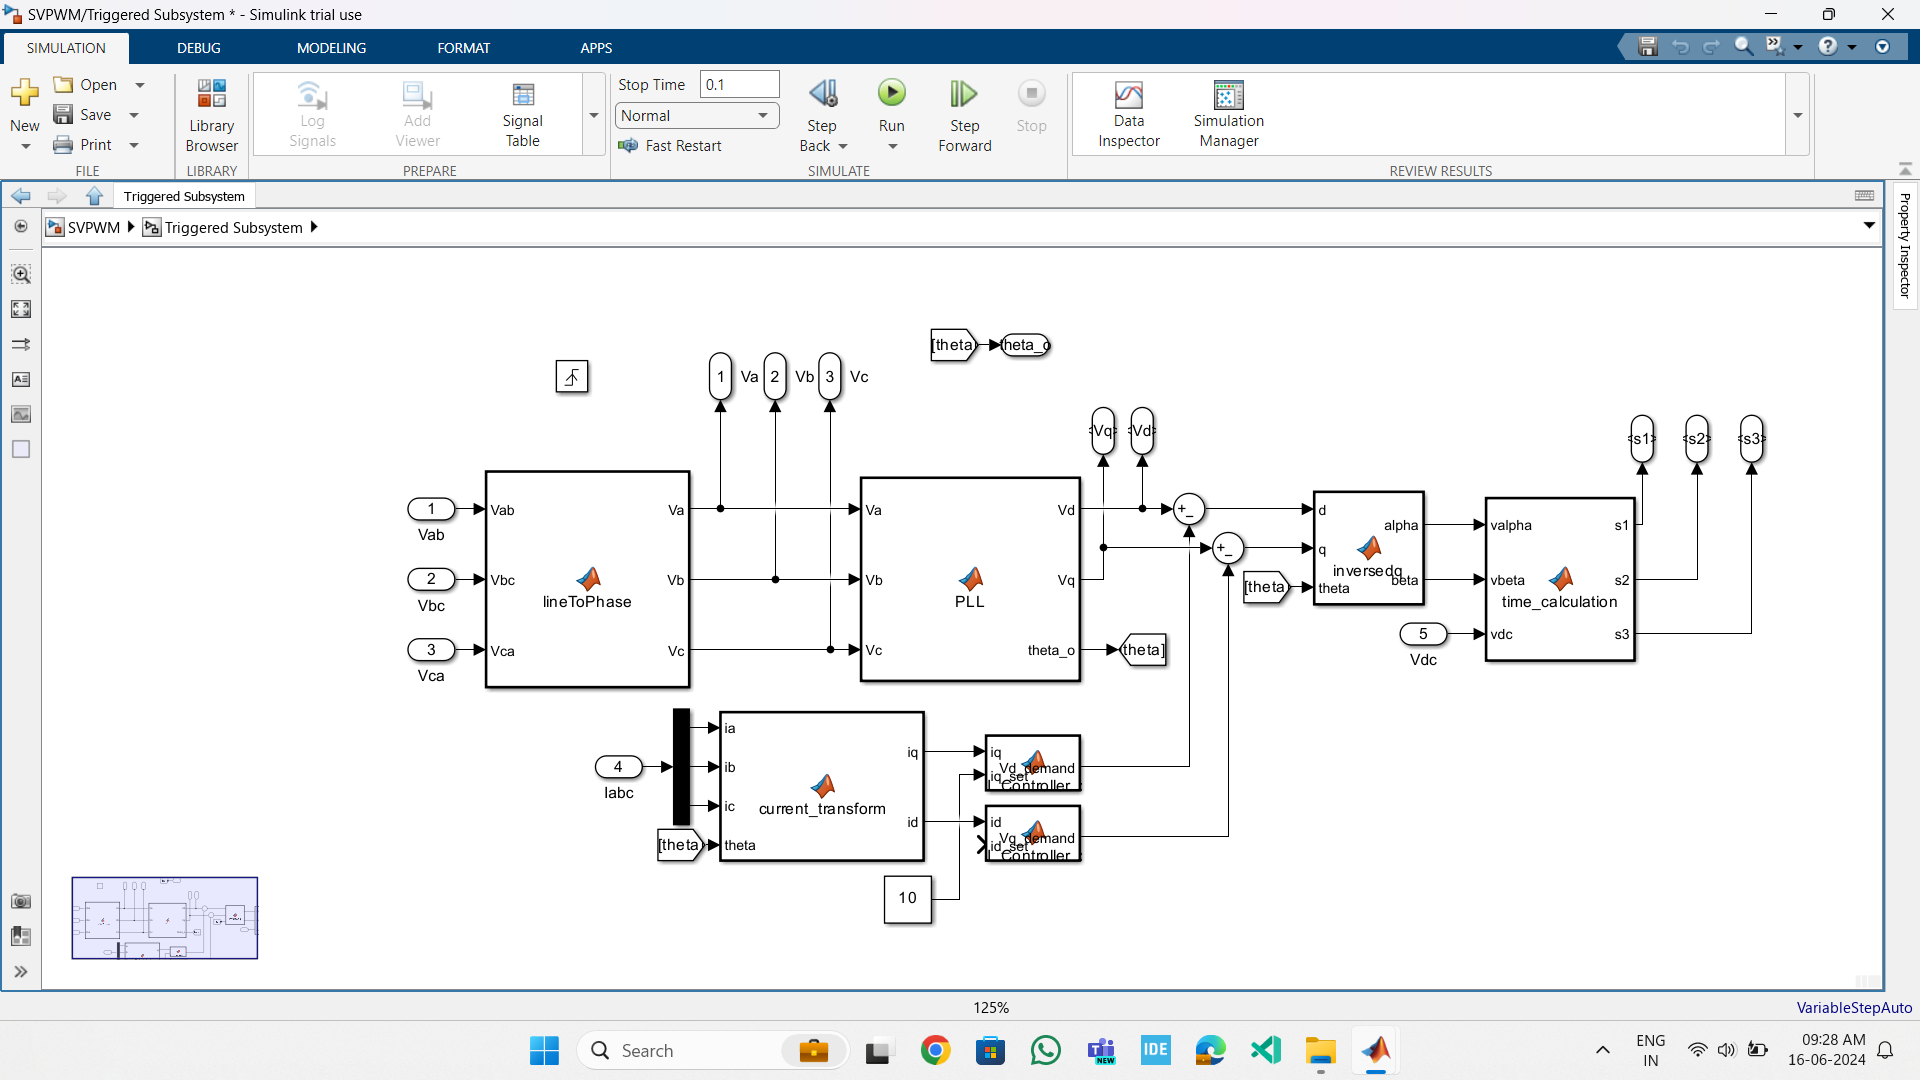
\includegraphics[width=\textwidth]{Control flow.png}
    \caption{Control System}
    \label{fig:Control System}
\end{figure}
\subsubsection{Voltage Transformation}
Transform the measured line voltages from the three-phase source into the
alpha-beta frame using the Clarke transform. This transformation facilitates
easier analysis and control of the three-phase system. The Clarke transform
converts three-phase voltages into two orthogonal components (alpha and beta),
simplifying the analysis of the system's dynamics and making it easier to
implement control strategies.

\subsubsection{Phase-Locked Loop (PLL)}
Incorporate a Phase-Locked Loop (PLL) block to convert the voltages from the
alpha-beta frame to the dq rotating reference frame. Additionally, the PLL
provides the angle theta of the voltage vector, crucial for subsequent control
strategies. The PLL ensures synchronization with the grid by maintaining a
constant phase relationship, which is vital for accurate control and stability
of the system.

\subsubsection{Current Measurement and Transformation}
Measure the line current flowing into the front end, and using Clarke and Park
transform blocks, convert it to the dq reference frame. Utilize the angle theta
obtained from the PLL for this transformation. The dq reference frame allows
for decoupled control of the direct and quadrature components of the current,
enabling more precise control of the active and reactive power.

\subsubsection{Current Regulation}
Regulate the current flowing into the front end to ensure stable operation and
adherence to system constraints. Employ two Proportional-Integral (PI)
controllers to compare the measured current to a predetermined set current
value and generate control signals for current regulation. The PI controllers
adjust the control signals to minimize the error between the measured and
desired current values, ensuring the system operates within the desired
parameters.

\subsubsection{Voltage Calculation and Transformation}
Add the control signals (delta Vq and delta Vd) obtained from the PI
controllers to the Vq and Vd components obtained from the PLL. Convert these
voltages back to the Clarke frame using the inverse Park transform. This step
integrates the control efforts with the system's voltages, transforming the
controlled voltages back into the stationary reference frame for further
processing and application.

\subsubsection{Gate Timing Calculation}
Utilize the voltages calculated in the previous step (V alpha* and V beta*) to
determine gate timings for the three-phase active front end. These gate timings
dictate the switching patterns of the Insulated Gate Bipolar Transistors
(IGBTs), essential for controlling the flow of current through the front end.
The precise timing of the IGBT switching is crucial for maintaining the desired
current and voltage waveforms, ensuring efficient and stable operation of the
power conversion system.

\subsection{Power System}
\begin{figure}[h]
    \centering
    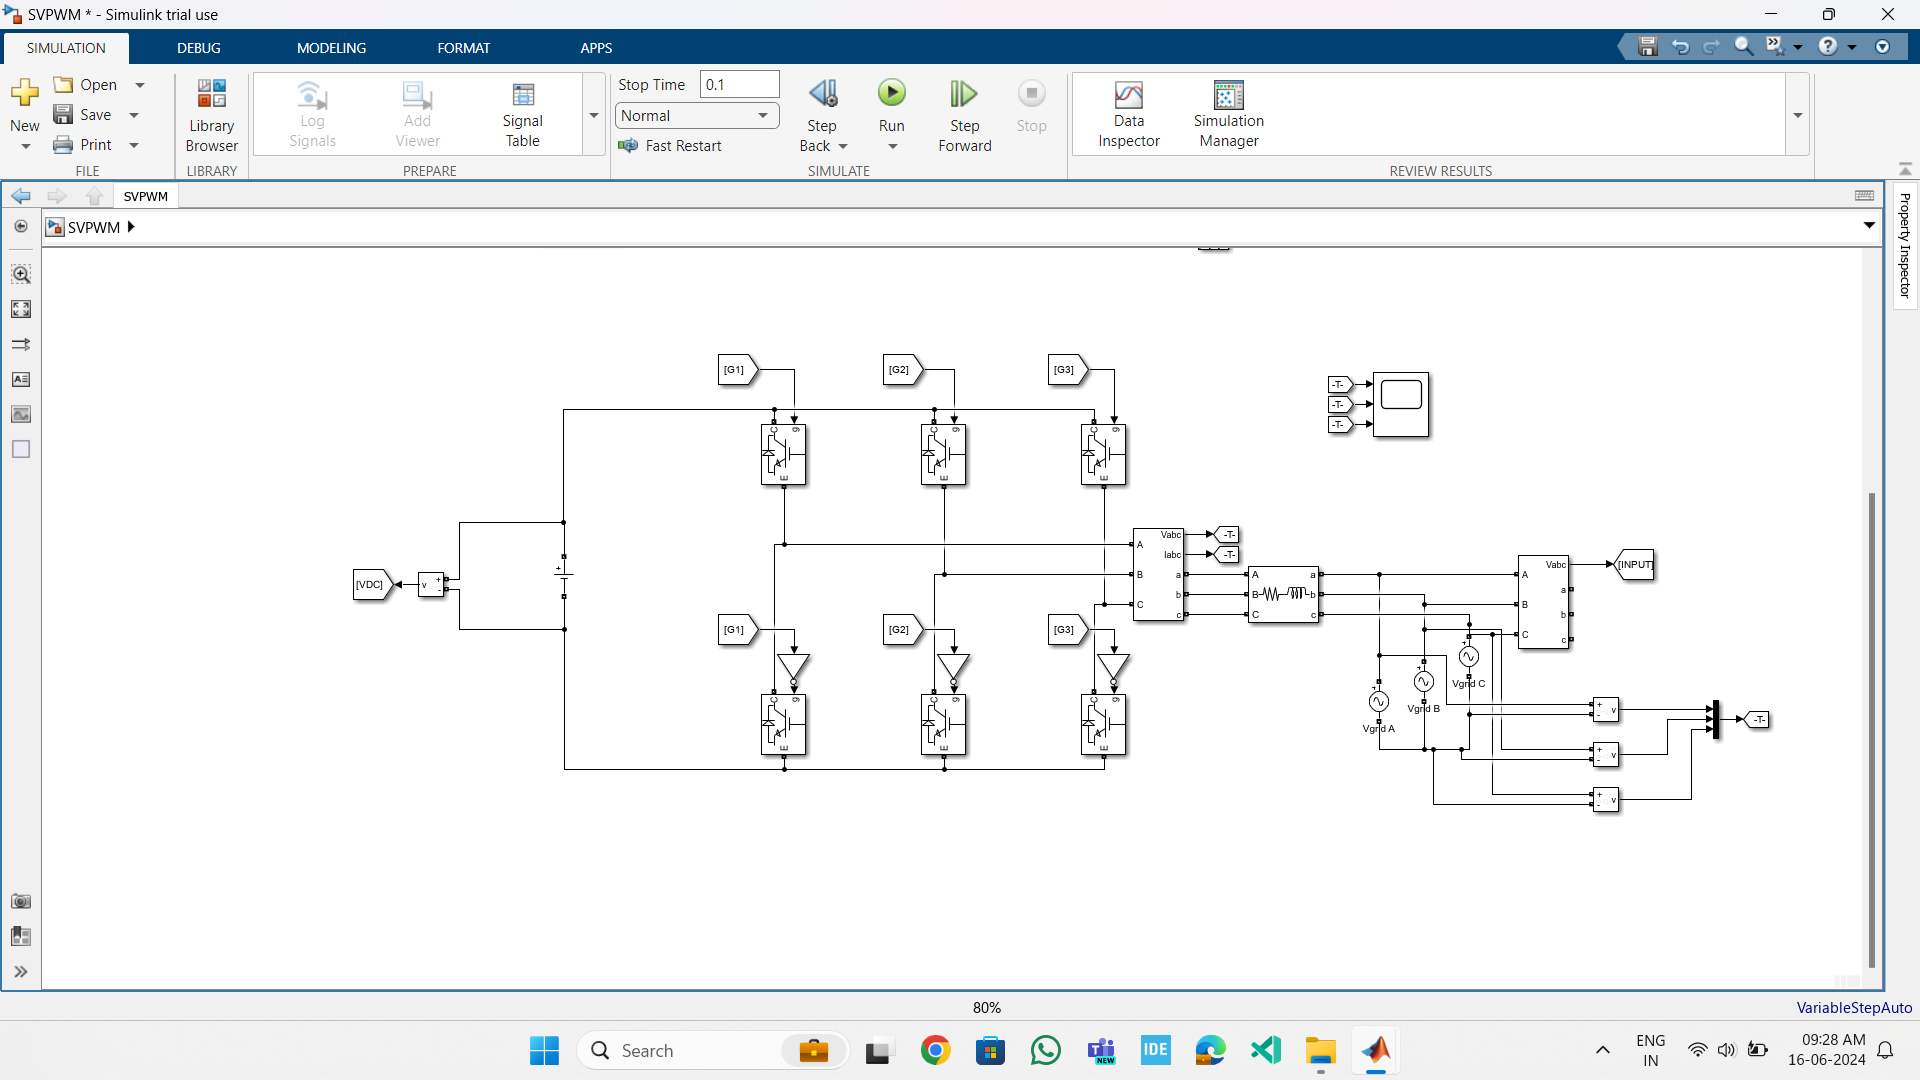
\includegraphics[width=\textwidth]{Power System.png}
    \caption{Power System}
    \label{fig:Power System}
\end{figure}

\subsubsection{Three-Phase AC Source}
The Three-Phase AC Source serves as the input power to the system.It provides
three sinusoidal voltage waveforms with a 120-degree phase difference between
each phase.The amplitude and frequency of the AC source are determined based on
the grid specifications or the application requirements.
\subsubsection{Three-Phase IGBT Bridge}
The Three-Phase IGBT Bridge is the primary power conversion and control element
in the system. It consists of six Insulated Gate Bipolar Transistors (IGBTs)
arranged in a three-phase bridge configuration. The IGBTs are switched in a
complementary manner to modulate the voltage across the load.

The IGBT bridge controls the flow of current from the AC source to the load by
switching the IGBTs on and off at precise intervals. This switching action
enables the conversion of AC power from the source to DC power, which can be
further conditioned or inverted as per the requirements of the application.

Additionally, the gate timing signals for the IGBTs are generated based on the
control signals calculated by the control system. These gate timing signals
dictate the switching pattern of the IGBTs, ensuring the desired current and
voltage waveforms are maintained for efficient and stable operation of the
power conversion system.

\section{Implementation}
\begin{figure}[h]
    \centering
    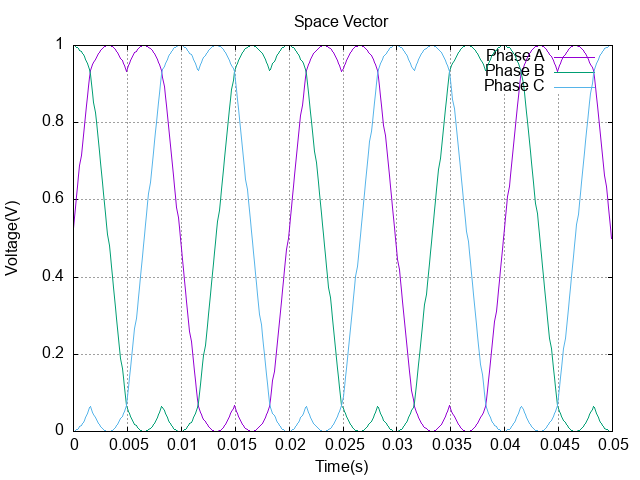
\includegraphics[width=\textwidth]{spacevector.png}
    \caption{Space Vector plotted using GNUPLOT}
    \label{fig:Space Vector Generated using C code}
\end{figure}
After completing the comprehensive simulation using Simulink/MATLAB to validate
the system design and control strategies, the project transitioned to the
implementation stage on a microcontroller. This phase focused on translating
theoretical concepts into practical application. This section includes the
selection process of the microcontroller, development of essential
transformation functions in C, and the integration of hardware components such
as timers, Direct Memort Access (DMA), and Analog to Digital Converter (ADC)
for accurate system monitoring and control.

\subsection{Microcontroller Selection}
The first step in the implementation phase was choosing an appropriate
microcontroller for the project. After evaluating several options, the
STM32F411 was selected due to its Digital Signal Processing (DSP) and Floating
Point Unit (FPU) capabilities. These features allowed us to run the
Proportional-Integral-Derivative (PID) loop at a high frequency of 10kHz,
providing 200 samples per cycle. This high sampling rate was crucial for
achieving precise control and stability in the system.

\subsection{Implementation of Voltage transform functions}
To handle the transformations required for the control algorithms, I
implemented the Clarke and Park transform functions in C. The process began by
creating an array with synthetic values to simulate the inputs. These values
were then fed into the custom transformation functions. The output was verified
using GNUPLOT to ensure the accuracy of the transformations. This step was
essential to validate the mathematical operations and ensure the functions were
performing as expected.

\subsection{Microcontroller Programming and Testing}
With the transformation functions ready, I proceeded to program the STM32F411
microcontroller. This phase involved a deep dive into various aspects of the
microcontroller, including timers, Direct Memory Access (DMA), and
Analog-to-Digital Converters (ADC).
\begin{itemize}
    \item \textbf{ADC Sampling}: I utilized the ADC to sample the voltage values from the system. This real-time data acquisition was critical for the subsequent control processes.
    \item \textbf{Transformation and Modulation}: The sampled voltage values were processed using the previously developed Clarke and Park transform functions. This step generated the necessary parameters for Space Vector Modulation (SVM).
\end{itemize}
\noindent
The integration of these components allowed for the generation of space vector
modulated waves, essential for controlling the power conversion system
effectively. Each part of this process was meticulously tested to ensure
reliability and accuracy, laying a strong foundation for the successful
deployment of the control system.